\documentclass[a4paper]{article}   

\usepackage[utf8]{inputenc}
\usepackage[english]{babel}

\usepackage{changepage}

\usepackage{tikz}
\usepackage{verbatim}
\usepackage{hyperref}

\usepackage{amsthm}
\newtheorem{theorem}{Theorem}[section]
\theoremstyle{definition}
\newtheorem{definition}{Definition}[section]

\title{Co-reference Resolution}
\author{Yohan Chalier}
\date{\today}

\renewcommand{\arraystretch}{1.2}

\newcommand{\sub}[1]{\textsubscript{#1}}
\newcommand{\hs}{\par\noindent\hspace{\parindent}}

\newenvironment{sentence}{\vspace{.1cm}\begin{adjustwidth}{2cm}{}\em}{\end{adjustwidth}\vspace{.1cm}}

\title{Co-reference resolution}
\date{\today}
\author{\textit{Yohan Chalier}\\ Symbolic Natural Language Processing (SD213) \\ \textsc{Télécom ParisTech}}


\begin{document}

\maketitle

\section{Problem positioning}

Co-reference occurs when two or more expressions refers to the same referent. Usually, one expression is in a full form (the \emph{antecedent}) and the other one in a abbreviated form (a \emph{proform}). For example:
\begin{sentence}
(1) The music\sub{1} was so loud that it\sub{1} couldn't be enjoyed.
\end{sentence}
Note that referring expressions are indexed with the same integer.

Co-reference resolution is needed to derive a correct interpretation of a text. Most algorithms simply look for the nearest preceding individual that is compatible with the referring expression. This compatibility comes from features unification, on features like gender or number. Such algorithm may correctly solve sentences like:
\begin{sentence}
(2) The girl\sub{1} likes her\sub{1} brother\sub{2} and protects him\sub{2}.
\end{sentence}
However, it will fail at differentiating sentences such as:
\begin{sentence}
(3) He\sub{1} said that John\sub{2} was coming. \\
(4) His\sub{1} sister said that John\sub{1} was coming.
\end{sentence}
In (3), \emph{He} cannot refer to \emph{John}, while in (4), such restriction do not apply. To thoroughly describe this phenomenon, one may use the following concepts of domination and c-command.

\begin{definition}[Parse tree]
An ordered, rooted tree that represents the syntactic structure of a string according to some context-free grammar.
\end{definition}

\begin{definition}[Domination]
Node $N_1$ dominates node $N_2$ if $N_1$ is above $N_2$ in the parse tree and one can trace a path from $N_1$ to $N_2$ moving only downwards in the tree (never upwards).
\end{definition}

\begin{definition}[c-command]
Node $N_1$ c-commands node $N_2$ if $N_1$ does not dominate $N_2$, $N_2$ does not dominate $N_1$ and the first (i.e. the lowest) branching node that dominates $N_1$ also dominates $N_2$.
\end{definition}

For example, in the tree showed in Figure \ref{fig:dummy_tree}, M does not c-commands any other node since it dominates all of them, whereas A c-commands B and all its children.

\begin{figure}
\centering
\begin{tikzpicture}
\node{M}
	child {node {A}}
	child {node {B}
		child {node {C} child {node {E}}}
		child {node {D}
			child {node {F}}
			child {node {G}}
		}
	};
\end{tikzpicture}
\caption{Dummy tree\label{fig:dummy_tree}}
\end{figure}

\begin{theorem}
\label{thm:ccommand}
One restriction between proform and antecedent is that the proform cannot appear in a position where it c-commands its antecedent.
\end{theorem}

This theorem explains the difference there is between \emph{"He said"} and \emph{"His sister said"}. As one can see in Figure \ref{fig:parse_tree_he_said}, the node \emph{He} c-commands the node \emph{John}, since they do not dominate each other and the first branching node that dominates \emph{He} is \emph{S} (\emph{NP} has only one child, it is not a branching node), and it dominates \emph{John}.

On the other hand, as shown in Figure \ref{fig:parse_tree_his_sister}, the first branching node that dominates \emph{His} is \emph{NP}, and it does not dominate \emph{John}, so \emph{His} does not c-command its antecedent. They can be associated together.

~\par

Finding a proof of Theorem \ref{thm:ccommand} is not trivial, and actually it has not been found at this day. This fact is just hypothesized. Some works try to interpret this with cognitive aspects \cite{bouchard2010explication}. The main issue with this rule is that the computational approach presents the result in a way it cannot be explained. Therefore people try to find other reasons to explain this phenomenon.

~\par

One hypothesis is the \emph{Novelty condition}: 
\begin{quote}
An anaphorically dependent element cannot have more determinate reference than its antecedent. \cite{wasow1979anaphora}
\end{quote}
This generalizes the c-command and seems to more a more cognitive explanation as it also handles external anaphorically relationships such as in (5) or (6):
\begin{sentence}
(5) The doctor\sub{1} walks in. The man\sub{1} keeps quiet. \\
(6) *The man\sub{1} walks in. The doctor\sub{1} keeps quiet.
\end{sentence}
Though, it may not handle all cases. And implementing this condition requires the computation of the determination of a reference, which is not trivial either.

\begin{figure}
\centering
\begin{tikzpicture}
\node{S}
	child {node[left=1cm] {NP}
		child {node {He}}		
		}
	child {node {VP}
		child {node {said}}
		child {node {SBAR}
			child {node {that}}
			child {node {S}
				child {node {NP} child {node {John}}}
				child {node[right=.5cm] {VP}
					child {node {was}}
					child {node {VP} child {node {coming}}}
				}
			}
		}
	};
\end{tikzpicture}
\caption{Parse tree of \emph{"He said that John was coming."}\label{fig:parse_tree_he_said}}
\end{figure}

\begin{figure}
\centering
\begin{tikzpicture}
\node{S}
	child {node[left=1cm] {NP}
		child {node {His}}		
		child {node {sister}}
		}
	child {node {VP}
		child {node {said}}
		child {node {SBAR}
			child {node {that}}
			child {node {S}
				child {node {NP} child {node {John}}}
				child {node[right=.5cm] {VP}
					child {node {was}}
					child {node {VP} child {node {coming}}}
				}
			}
		}
	};
\end{tikzpicture}
\caption{Parse tree of \emph{"His sister said that John was coming."}\label{fig:parse_tree_his_sister}}
\end{figure}

\section{Implementation}

The goal here is an implementation of a parser that solves co-reference, and rewrites the given sentence with indexes to identify the referencing groups. The final version of the Python script I wrote is available on GitHub \cite{github}.

\paragraph{Prolog struggles} My first idea was to re-use the CYK parser from the lab work on parsing. Though, inserting new pieces of code within the already done parser turned out more difficult than expected. I tried to take inspiration from the lab work on semantics processing with a predicate \texttt{refers(,)}. In the end, I was spending more time on debugging than actually working on co-reference. Therefore, I pivoted to Python.

\subsection{Grammar and lexicon}

I used English grammar and vocabulary. I followed the same pattern as in the lab works. Here is my grammar file:
\begin{verbatim}
    s --> np, vp
    np --> n
    np --> det, n
    np --> pn, n
    np --> pn
    vp --> v, np
    vp --> v, sub
    sub --> p, n, v
    vp --> vp, p, vp
\end{verbatim}
And here is my lexicon:
\begin{verbatim}
    n --> boy[gender:male;num:sing],
          sister[gender:female;num:sing],
          John[gender:male;num:sing],
          girl[gender:female;num:sing],
          brother[gender:male]
    det --> the
    pn --> his[gender:male;num:sing],
           her[gender:female;num:sing],
           he[gender:male], him[gender:male]
    v --> likes, protects, said, was_coming
    p --> and, that
\end{verbatim}
I used only two features, gender and number. Two functions, \texttt{read\_grammar} and \texttt{read\_lexicon}, process those files and produces Python dictionaries. Keys are the left part of the rules, values are a lists of the split right part. Features are also stored as a dictionary.

\subsection{Parser}

I implemented my own version of a simple top-down parser. Everything is achieved within a class \texttt{Parser}. The method \texttt{parse\_aux} iterates through the grammar rules and stops when the end of the sentence is reached. It uses recursion to try to parse smaller portions of the sentence.

Along the way, it produces the parse tree as an instance of the class \texttt{Node}, which is a recursive data type. Nodes store a label and a list of references of its children. Other attributes are stored, such as a reference to the parent. The Figure \ref{fig:screenshot} is an example of an outputted parse tree for the sentence (2).

\begin{figure}
\centering
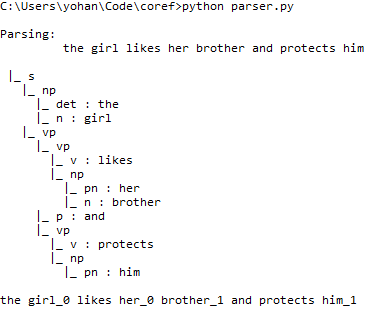
\includegraphics[scale=1]{screenshot_parse_tree}
\caption{Screenshot of the outputted parse tree\label{fig:screenshot}}
\end{figure}

\subsection{Co-reference}

In this script, I focused on the c-command condition and features agreement. The use of the class \texttt{Node} makes co-reference resolution rather easy. The computation of domination is actually a search function in a recursive structure, since we only need to check whether the dominated target is within the offspring of the dominant one, which is easy to compute:
\begin{verbatim}
def dominates(self, other):
    """ Returns True if 'self' dominates 'other' """

    if len(self.childs) == 0:  # bottom of the tree,
        return False           # 'other' was not found

    for child in self.childs:  # recursive iteration
        if child == other or child.dominates(other):  
            return True
    return False
\end{verbatim}
Then, the \texttt{c\_commands} method climbs up the tree until a branching node is found, and then uses the domination to return the answer:
\begin{verbatim}
def c_commands(self, other):
    """ Returns True if 'self' c-commands 'other' """

    # first we make sure no one dominates the other
    if self.dominates(other) or other.dominates(self):
        return False

    parent = self.parent
    while parent is not None:  # tree climbing
        if len(parent.childs) > 1 and parent.dominates(self):
            return parent.dominates(other)
        parent = parent.parent
    return False
\end{verbatim}


Then, once the parse tree has been computed, for each word recognized as a referring expression (for now, only pronouns), a method of the \texttt{Parser} finds a compatible word (\emph{features agreement}), and if the proform does not c-command that word, it links them both. Results are the following:

\begin{verbatim}
     Parsing: he said that John was_coming
     he_0 said that John was_coming

     Parsing: his sister said that John was_coming
     his_0 sister said that John_0 was_coming

     Parsing: the girl likes her brother and protects him
     the girl_0 likes her_0 brother_1 and protects him_1
\end{verbatim}

\section{Conclusion}
Although the script works on the sentences (2), (3) and (4), it does not scales up easily. The top-down parser is really flawed and breaks easily. Using the NLTK parser \cite{nltk} would solve this. Features can be added directly to the lexicon, the unifier used in the script deals with abstract features instances. A great improvement could rely on the implementation of the Novelty condition.

\bibliography{references}
\bibliographystyle{unsrt}

\end{document}
